\documentclass[german,a4paper, 12pt]{llncs}
\usepackage[left=30mm,right=30mm,top=25mm,bottom=25mm]{geometry}
\setlength{\footskip}{6mm} % Abstand Seitenzahl zu Text
\setcounter{tocdepth}{2}
\setcounter{secnumdepth}{6}
\makeatletter
\renewcommand*\l@author[2]{}
\renewcommand*\l@author[2]{}
\makeatletter
\usepackage[utf8]{inputenc}
\usepackage[backend=biber,sorting =none]{biblatex}
\usepackage{csquotes}
\usepackage{graphicx}
\usepackage{babel}

\usepackage{parskip}
\usepackage{float}

%\usepackage{hyperref}
\usepackage{filecontents}


\begin{filecontents}{references.bib}
	
	@article{introToCNN,
		author = {O'Shea, Keiron and Nash, Ryan},
		year = {2015},
		month = {11},
		pages = {},
		title = {An Introduction to Convolutional Neural Networks},
		journal = {ArXiv e-prints}
	}
	@article{surveyOfDeepLearing,
		author = {Jiao, Licheng and Zhang, Fan and Liu, Fang and Yang, Shuyuan and Li, Lingling and Feng, Zhixi and Qu, Rong},
		year = {2019},
		month = {09},
		pages = {1-1},
		title = {A Survey of Deep Learning based Object Detection},
		volume = {PP},
		journal = {IEEE Access},
		doi = {10.1109/ACCESS.2019.2939201}
	}
	
	@ONLINE{spatialMapping,
		title = {Spatial Mapping},
		url = {https://docs.microsoft.com/de-de/windows/mixed-reality/spatial-mapping},
		urldate = {2020-04-17},
	}
	
	@ONLINE{spatialMappingUnity,
		title = {Räumliche Zuordnung in Unity},
		url = {https://docs.microsoft.com/de-de/windows/mixed-reality/spatial-mapping-in-unity},
		urldate = {2020-04-17},
	}
	
	@INPROCEEDINGS{cNNforClass,
		author={N. {Jmour} and S. {Zayen} and A. {Abdelkrim}},
		booktitle={2018 International Conference on Advanced Systems and Electric Technologies (IC ASET)}, 
		title={Convolutional neural networks for image classification}, 
		year={2018},
		volume={},
		number={},
		pages={397-402},}
	
	%https://docs.microsoft.com/de-de/learn/modules/analyze-images-computer-vision/2-image-analysis-azure
	
	@ONLINE{getAzure,
		title = {Microsoft Azure Computer Vsion},
		url = {https://azure.microsoft.com/en-us/services/cognitive-services/computer-vision/},
		urldate = {2020-06-12},
	}
	@ONLINE{whatIsAzure,
		title = {What is Computer Vision},
		url = {https://docs.microsoft.com/en-us/azure/cognitive-services/computer-vision/home},
		urldate = {2020-06-12},
	}
	@ONLINE{objDetectAzure,
		title = {Detect common objects in images},
		url = {https://docs.microsoft.com/en-us/azure/cognitive-services/computer-vision/concept-object-detection},
		urldate = {2020-06-12},
	}
	
	@ONLINE{pytorch,
		title = {From research to production},
		url = {https://pytorch.org/},
		urldate = {2020-06-12},
	}
	@ONLINE{Azure302Doc,
		title = {Mr und Azure 302 Maschinelles Sehen},
		url = {https://docs.microsoft.com/de-de/windows/mixed-reality/mr-azure-302},
		urldate = {2020-06-12},
	}
	@ONLINE{Azure302bDoc,
		title = {Mr und Azure 302b benutzerdefinierte Vision},
		url = {https://docs.microsoft.com/de-de/windows/mixed-reality/mr-azure-302b},
		urldate = {2020-06-12},
	}
	@INPROCEEDINGS{cars,
		author={X. {Chen} and H. {Ma} and J. {Wan} and B. {Li} and T. {Xia}},
		booktitle={2017 IEEE Conference on Computer Vision and Pattern Recognition (CVPR)}, 
		title={Multi-view 3D Object Detection Network for Autonomous Driving}, 
		year={2017},
		volume={},
		number={},
		pages={6526-6534},
	}
	@ONLINE{mlluminfeatures,
	title = {Magic Leap Features},
	url = {https://developer.magicleap.com/en-us/learn/guides/magic-leap-features},
	urldate = {2020-09-18},
	}
	@ONLINE{mlluminOS,
	title = {Lumin OS Overview},
	url = {https://developer.magicleap.com/en-us/learn/guides/lumin-os-overview},
	urldate = {2020-09-18},
}
	@ONLINE{mlluminOS,
	title = {Lumin OS Overview},
	url = {https://developer.magicleap.com/en-us/learn/guides/lumin-os-overview},
	urldate = {2020-09-18},
}
	@ONLINE{mlluminworldreconstruktion,
	title = {World Reconstruktion},
	url = {https://developer.magicleap.com/en-us/learn/guides/world-reconstruction-overview-landing},
	urldate = {2020-09-18},
}
	@ONLINE{mlmeshingunity,
	title = {1.4 Spatial Meshing - Unity},
	url = {https://developer.magicleap.com/en-us/learn/guides/meshing-in-unity},
	urldate = {2020-09-18},
}
	@ONLINE{mlappsecurity,
	title = {App Security},
	url = {https://developer.magicleap.com/en-us/learn/guides/application-security-overview},
	urldate = {2020-09-18},
}
	@ONLINE{mlofficialsalespitch,
	title = {magic leap 1},
	url = {https://www.magicleap.com/en-us/magic-leap-1},
	urldate = {2020-09-18},
}
	@ONLINE{mlglossary,
	title = {Glossary and Usage},
	url = {https://developer.magicleap.com/en-us/learn/guides/glossary},
	urldate = {2020-09-18},
}

	@ONLINE{unitycameratoworldmatrix,
	title = {Camera.cameraToWorldMatrix},
	url = {https://docs.unity3d.com/ScriptReference/Camera-cameraToWorldMatrix.html},
	urldate = {2020-09-18},
}

	@ONLINE{unitymultiplyoint,
	title = {Matrix4x4.MultiplyPoint},
	url = {https://docs.unity3d.com/ScriptReference/Matrix4x4.MultiplyPoint.html},
	urldate = {2020-09-18},
}
	@ONLINE{azureobjdetec,
	title = {Erkennen von alltäglichen Objekten in Bildern},
	url = {https://docs.microsoft.com/de-de/azure/cognitive-services/computer-vision/concept-object-detection},
	urldate = {2020-09-24},
}	
	@ONLINE{fromjson,
	title = {JsonUtility.FromJson},
	url = {https://docs.unity3d.com/ScriptReference/JsonUtility.FromJson.html},
	urldate = {2020-09-24},
}	

\end{filecontents}

\addbibresource{references.bib}
\title{Bachelorarbeit}
\subtitle{Automatisches Labeln von Objekten in einer Augmented Reality Umgebung}
\author{\parbox{.9\textwidth}{\centering 
		\large Janelle Pfeifer \\
		\small Delpstraße 28\\
		53359 Rheinbach \\
		janelle.pfeifer@smail.inf.h-brs.de}}
\institute{\parbox{.9\textwidth}{\centering 
		\large Hochschule Bonn-Rhein-Sieg \\
		\normalsize Institute of Visual Computing \\ 
		\small Fachbereich Informatik \\
		Studiengang: Informatik (B.SC.)\\
		\phantom{.}\\
		\normalsize Erstprüfer: Prof. Dr. Ernst Kruijff\\
		\normalsize Zweitprüfer: Prof. Dr. André Hinkenjann\\
		\phantom{.}\\
		\normalsize Rheinbach, 1.10.2020}}
\begin{document}
	
%{\let\newpage\relax\maketitle}
\maketitle
\newpage
\section*{Selbstständigkeitserklärung}
\newpage
\section*{Zusammenfassung}
Für Viele Augmented Reality Anwendungen ist es sehr wichtig das die Gegenstände in der Umgebung bekannt sind, damit mit ihnen Interagiert werden kann. 
	
Für Große und sich verändernde Umgebungen ist es sehr arbeitsaufwändig da der Nutzer das im Grunde einzeln machen muss.

In dieser Arbeit wird ein Verfahren vorgestellt, mit dem Gegenstände Automatisch erkannt werden können. Es werden Bilder von der realen Umgebung aufgenommen und mithilfe von Image Based Object Detection analysiert. Die Erkannten Objekte werden dann in der Augmented Reality Umgebung lokalisiert und mit einem Label markiert. 
	
\newpage
\tableofcontents
\newpage
\section{Einleitung}
%noch ein bsichen lang. kann die beschreibung der zwei schlechteren methoden verkürzen. Abschnitte 2 3 4 

Augmented Reality (AR) ist eine Vermischung der realen Welt mit digitalen Elementen. Es wird durch Anzeigegeräte, wie Handys, Tablets oder Augmented Reality Brillen, präsentiert und bietet ein intuitives Benutzerinterface, um Informationen über Objekte der realen Welt anzuzeigen. Dafür muss erfasst werden, welche Gegenstände sich in der Umgebung befinden. %müssen Informationen über die Umgebung erfasst werden. %Es ist wichtig zu bestimmen welche Objekte sich in der Umgebung befinden, die durch AR erweitert werden soll.

%wie wird objekt erkennung gemacht
Es gibt mehrere Möglichkeiten Gegenstände zu erkennen. Zum einen können Markierungen in der realen Welt verwendet werden. Dabei handelt es sich um statische Bilder, beispielsweise ein Foto, oder ein QR Code, die von einer Kamera eingescannt werden. Der Marker ist einzigartig für jedes Objekt, damit sie voneinander unterschieden werden können. Der Nachteil bei diesem Vorgehen ist der Arbeitsaufwand, der damit verbunden ist, jeden Gegenstand einzeln zu markieren.% und die Bedeutung der AR Applikation die Marker bekannt zu machen. 
%Außerdem können Marker leicht verdeckt werden und nicht an jedes Object lassen sich Marker anbringen. 

Wenn man Markierungen in der realen Welt umgehen möchte, kann man den Nutzer der Applikation bitten, beispielsweise per Geste auf Objekte der realen Welt zu weisen, die erkannt werden sollen. Für jedes der Objekte muss der Nutzer angeben, um welche Art von Gegenstand es sich handeln, damit die Applikation unterschiedliche Objekte auseinander halten kann und die korrekten Informationen mit ihren assoziiert. Auch hier ist der Arbeitsaufwand hoch.

%also basically per hand. was ziemlich schlecht ist. % es bleibt nur übrig automatisch zu tracken
Beide der Verfahren lassen sich schlecht skalieren um große AR Umgebungen abzudecken. Nur eine vollautomatische Objekterkennung ist skalierbar. 

%object detection funktoniert was bilder angeht.
Um diese Automatisierung zu erreichen, kann Image based Object Detection aus dem Bereich der Computer Vision verwendet werden.
Dieses Verfahren ist darauf ausgelegt Objekte in Bildern zu erkennen.\cite{introToCNN}

%Diese Automatisierung wollen wir in dieser Thesis mit einer Hololens durchführen. quasi zeigen das es geht.
In dieser Thesis wird das Erkennen und Labeln von Objekten in einer AR Umgebung, mithilfe von Image based Objekt Detection, automatisiert. 
Das AR Gerät Magic Leap Lightwear wird als Benutzerinterface und Plattform verwendet.


%todo Motivation und Ziele. MinmimalZiel, Maximalzielt etc

\section{Related Work}

%todo

\section{Grundlagen}

%\subsection{Computervision}
%In dem Bereich der Bildverarbeitung gibt es viele Algorithmen, die es ermöglichen Objekte in einem Bild erkennbar zu machen und zu verarbeiten.
%todo computer vision erklären ?


\subsection{Grundlagen zu Augmented Reality}
\subsubsection{Augmented Reality} %Einfürhung in AR
%todo
Augmented Reality (AR) ist eine Vermischung der realen Welt mit digitalen Elementen. Es wird durch Anzeigegeräte, wie Handys, Tablets oder Augmented Reality Brillen, präsentiert und bietet ein intuitives Benutzerinterface, um Informationen über Objekte der realen Welt anzuzeigen. Dafür muss erfasst werden, welche Gegenstände sich in der Umgebung befinden. %müssen Informationen über die Umgebung erfasst werden. %Es ist wichtig zu bestimmen welche Objekte sich in der Umgebung befinden, die durch AR erweitert werden soll.

\subsubsection{View Management}
%todo

\subsection{Spatial Mapping} 
Durch Spatial Mapping wird eine 3D Abbildung der realen Welt erschaffen. So können Hologramme mit der Umgebung interagieren, diese verdecken oder von ihr verdeckt werden.\cite{spatialMapping} 

\subsection{Magic Leap AR Brille}

Die Magic Leap Lightwear ist eine Augmented Reality Brille. Sie besitzt neun Sensoren und mehrere Kameras. Dazu gehören:
\begin{itemize}
	\item ein Infrarot Tiefen-Sensor,
	\item ein Eye Tracker,
	\item eine Foto und Video Kamera, die im Format 16:9 mit einer Auflösung von 1920 x 1080 Pixeln aufnehmen,
	\item Umgebungskameras die in unterschiedliche Richtungen ausgerichtet sind. \cite{mlofficialsalespitch,mlglossary}
\end{itemize}

Der Output geschieht über ein Display mit einem 50 Grad Field of View und einem Seitenverhältnis von 4:3. 
Eingaben erfolgen über einen 6 Degree of Freedom Controller.\cite{mlofficialsalespitch,mlglossary}

Die Magic Leap Brille läuft auf dem Betriebssystem Lumin OS. Dieses wurde für Augmented Reality entwickelt und bietet Applikationen entsprechende Funktionalitäten an. Beispielsweise führt das Betriebsamstem Spatial Mapping durch.\cite{mlluminOS,mlluminfeatures}

Dabei werden mit den Sensoren und Kameras der Brille Daten aufgenommen und in einen zeitlichen Zusammenhang mit der Bewegung der Brille gesetzt, um eine Rekonstruktion des Raumes zu erhalten.\cite{mlluminOS,mlluminfeatures,mlluminworldreconstruktion,mlmeshingunity}

Lumin OS bietet es Applikationen an,
\begin{itemize}
	\item Raycast auf die Umgebung durchzuführen und
	\item ein Mesh der Rekonstruktion zu erhalten.
\end{itemize}
%todo was ist ein raycast?
Neben dem Spatial Mapping unterstützt Lumin OS das Verarbeiten vom Input des Controllers und verwaltet die Zugriffsrechte der Applikationen. Dazu gehört beispielsweise der Zugriff auf die Fotokamera und das Netzwerk.\cite{mlluminfeatures,mlappsecurity}

\subsection{3D Computergrafik}

\subsubsection{Lokale und globale Koordinatensysteme in 3D Szenen}
%\newline
In einer 3D Szenen werden die Positionen von Objekten als Matrizen in dreidimensionalen Koordinatensystemen verwaltet.
Es gibt ein globales Koordinatensystem (auch Weltkoordinatensystem oder World Space), in dem alle Objekte relativ zu einem gewählten Ursprung liegen. 

Jedes Objekt hat zusätzlich ein eigenes, lokales Koordinatensystem (Objektkoordinatensystem). Dessen Ursprung liegt in dem jeweiligen Objekt.
Die Position und Rotation des Objektes in dem globalen Koordinatensystem bestimmt die Relation zwischen dem globalen und dem lokalen Koordinatensystem. 

Das lokale Koordinatensystem einer Kamera wird auch Camera Space genannt. Die Relation zwischen dem Camera Space und dem globalen Koordinatensystem wird in Unity durch die cameraToWorld Matrix beschrieben. Mithilfe dieser Matrix kann eine Koordinate aus dem Camera Space in die entsprechende Koordinate des globalen Koordinatensystems transformiert werden.\cite{unitycameratoworldmatrix}

Dazu wird die Koordinate als Vektor angegeben und mit der cameraToWorld Matrix multipliziert. Das Resultat ist ein Vektor, der eine Koordinate im globalen Koordinatensystem angibt.\cite{unitycameratoworldmatrix,unitymultiplyoint}

\subsubsection{Kamera in 3D-Computergrafik}
\paragraph{View Frustum}
ist das Teilvolumen einer 3D Szene, die auf den zweidimensionalen Bildschirm abgebildet wird. Alle Objekte die von der Kamera gesehen werden, befinden sich in dem View Frustum.

\paragraph{Clipping Plane}
bezeichnet eine Ebene, die den View Frustum quer zur Blickrichtung begrenzt. 
Es gibt eine vordere und eine hintere Clipping Plane.
Die vordere Clipping Plane liegt nah an der Kamera. Alle Objekte die zwischen der Kamera und der vorderen Clipping Plane liegen, werden nicht angezeigt.

Die hintere Clipping Plane limitiert wie weit Objekte entfernt sein können, bevor sie nicht mehr zu sehen sind.

%to myself: yay :) you're doing well I believe in you!

\subsection{Computer Vision}
\subsection{Object Detection}
Objekt Detection ist eine Aufgabe der Computer Vision. Es sollen Objekte in einem Bild erkannt werden. 
Für die Objekte wird eine Klasse und eine Bounding Box bestimmt. 
Die Klasse gibt an, um welche Art von Objekt es sich handeln. Beispielsweise ob es eine Tastatur oder ein Computerbildschirm ist.
Die Bounding Box gibt ein Viereck auf dem Bild an, in dem sich das Objekt befindet.

\subsection{Artificial Neural Networks}
Artificial Neural Networks sind Machine Learning Architekturen. Sie können beispielsweise Musik, Text oder Bilder nach Mustern durchsuchen. Sie sind für keine genaue Aufgabe programmiert, sondern lernen indem sie mit Beispieldaten trainiert werden. 

Für jedes Beispiel gibt es ein Label, das angibt ob es das gesuchte Muster enthält oder nicht. Die Struktur des Networks verfügt über Gewichte, die Einfluss auf den Output haben. Mit jedem Trainingsbeispiel passt das Network die Gewichte an, sodass der Output dem Label des Beispiels entspricht.\cite{introToCNN,surveyOfDeepLearing}

%Artificial Neural Networks bestehen aus einer Menge an verbundenen Knoten, die jeweils eine Berechnung durchführen. Diese Knoten sind in Ebenen aufgeteilt, den Input Layer, den Output Layer, und mehrere Hidden Layer dazwischen. Die Knoten einer Ebene sind mit allen Knoten der Vorherigen Ebene verbunden.\cite{introToCNN,surveyOfDeepLearing}
%Das Neural Network bekommt eine Menge an Daten als Input. Die Knoten arbeiten zusammen um den Output zu erzeugen. Dabei wird über Gewichte entschieden, wie viel Einfluss das Ergebnis der einzelnen Knoten auf die nächste Ebene hat.\cite{introToCNN,surveyOfDeepLearing}
%Um ein Neural Network zu trainieren, wird der Output von einem Mensch bewertet. Das Neural Network nutzt diese Bewertung, um die Gewichte der einzelnen Knoten zu verändern. So passt sich das Neural Network an. \cite{introToCNN,surveyOfDeepLearing}

\subsection{Convolutional Neural Networks}
Convolutional Neural Networks sind auf das Verarbeiten von Bildern spezialisiert. Sie nutzen aus, das Bilder viele Redundanzen und informationsarme Bereiche haben. Daher können mit jedem Verarbeitungsschritt des Networks Informationen weggelassen werden. So können Rechenzeit und Volumen der Trainingsdaten verringert werden.\cite{introToCNN,surveyOfDeepLearing,cNNforClass}

%So wird das Convolutional Neural Network gezwungen sich auf wesentliche Teile des Bildes zu knozentrieren. Mit jedem verarbeitungsschritt sinkt die Menge an Informationen, die Das Sie Brauceh weniger Rechenzeit und weniger Trainigsdaten als ein generelles Artificial Neural Network werden eingesetzt um Muster in Bildern zu erknenne

%Convolutional Neural Networks sind Machine Learning Architekturen, die darauf ausgelegt sind, Muster in Bildern zu erkennen. Sie müssen auf das Muster trainiert werden. Dazu wird ihnen eine Menge an Bildern, die Teilweise das Muster erhalten, und der gewünschte Output, der erreicht werden soll, gegeben. Die Struktur des Network verfügt über Gewichte, die die Berechnung des Outputs beeinflussen. Mit jedem Trainigsbild passt das Network die Gewichte an, damit es die Mustern korrekt erkennen kann.\cite{introToCNN,surveyOfDeepLearing}

%Convolutional Neural Networks werden hauptsächlich eingesetzt um Muster in Bildern zu erkennen. Daher ist ihre Struktur und ihre Arbeitsweise auf Bilder spezialisiert. Sie brauchen weniger Rechenzeit und weniger Trainingsdaten als ein generelles Artificial Neural Network für dieselbe Aufgabe brauchen würde.\cite{introToCNN,surveyOfDeepLearing,cNNforClass} 
%Die Knoten in einer Ebene eines Convolutional Neural Network sind nur mit wenigen Knoten der vorherigen Ebene verbunden. So sinkt die Menge an Informationen mit jeder Ebene. Das CNN wird gezwungen sich auf wesentliche Teile des Bildes zu konzentrieren, mit denen beispielsweise ein Objekt oder  Muster erkannt werden kann. \cite{introToCNN,surveyOfDeepLearing}


\subsection{REST Anfragen}
todo
REST, was ist eine API, POST, Repsonse, ResponceCode
%todo: this

\subsection{Azure Computer Vision}
Microsoft Azure bietet einen Computer Vision Service an. Dabei handelt es sich um mehrere KIs, die für unterschiedliche Aufgaben trainiert wurden. Dazu gehört unter anderem ein Service für Object Detection.

Dabei sendet der Anwender ein Bild an Microsoft, dort wird es verarbeitet und ein Ergebnis zurückgeschickt.\cite{getAzure,whatIsAzure,objDetectAzure,Azure302Doc}

Die Object Detection basiert auf einem trainierten KI Modell. Dieses kann nur Objekte erkennen, für die es trainiert wurde.
Zusätzlich können Objekte, die in dem Foto sehr klein sind oder nah bei anderen Objekten liegen, nicht erkannt werden.\cite{azureobjdetec}

Der Service ist durch eine REST-API erreichbar. Mit einer Post Anforderung werden die Bilddaten übertragen und die Analyse angefragt. Die Response Nachricht beinhaltet eine Json-Datei, welche die gefundene Objekte und deren Positionen auf dem Foto beinhaltet. 
%Um den Service zu nutzen wird eine Http Post Anforderung an die WebAdresse geschickt. 

%{"objects":[{"rectangle":{"x":1377,"y":900,"w":157,"h":138},"object":"computer mouse","confidence":0.681},{"rectangle":{"x":1336,"y":0,"w":584,"h":841},"object":"display","confidence":0.873},{"rectangle":{"x":315,"y":25,"w":906,"h":622},"object":"display","confidence":0.839},{"rectangle":{"x":447,"y":800,"w":862,"h":166},"object":"computer keyboard","confidence":0.71}],"requestId":"a77e261a-7d40-4159-bf78-19d8fb61ad92","metadata":{"height":1080,"width":1920,"format":"Jpeg"}}

\subsection{Azure Custom Vision}
Azure bietet zusätzlich einen Computer Vision Service an, den der Nutzer trainieren kann. Custom Vision kann dann verwendet werden, wenn Azure Object Detection für Objekte nicht trainiert ist.\cite{Azure302bDoc}


dass es sich bei einem erkannten Objekt tatsächlich um eine Nivea Dose handelt


todo: was ist die Prediction? 
Erkälre die Iterations
Erkläre was die Genauigkeit der Predation aussagt.
%todo write more about this



\section{Design}
%todo SoftwareDesign mit Diagrammen. strukturierter aufbauen.

Das Ziel ist das Erkennen und Labeln von Objekten in einer AR Umgebung, durch Image Based Objekt Detection.

Wenn der Nutzer das Signal gibt, beginnt die Detection. Als Erstes wird ein Foto mit der Kamera der AR Brille aufgenommen. 
Dieses Foto wird dann an Azure Object Detection und Azure Custom Vision geschickt. 
Die Services untersuchen das Foto nach Objekten, geben deren Klasse und Position auf dem Foto an.

Für jedes Objekt soll eine Markierung erstellt werden, die zeigt wo sich das Objekt in der realen Welt befindet.
Dafür wird in der 3D Szene der AR Umgebung eine virtuelle Repräsentation des Fotos erschaffen. Die Fotorepräsentation muss die richtige Skalierung, Position und Rotation haben, um das räumliche Verhältnis zwischen der realen Foto-Kamera und der Umgebung nachzubilden.

Da die Foto-Kamera und das Display nahe beieinander liegen und den gleichen Blickwinkel haben, kann die Position des Displays als Repräsentation des Fotos genutzt werden. In der 3D Szene ist das Display mit der Hauptkamera gleichgesetzt. Die Clipping Plane der Kamera hat somit die gleiche Rotation und eine zumindest ähnliche Position und Skalierung wie das Foto. 

Daher werden die Foto-Positionen auf Koordinaten der Clipping Plane abgebildet. Dabei werden verbleibende Positions- und Skalierungs-Unterschiede ausgeglichen. Für jedes Objekte wird so eine Koordinate auf der Clipping Plane bestimmt. 

Als Nächstes wird ein Raycast, von der Kamera aus, durch die Clipping Plane Koordinate geschickt. Der Raycast schneidet sich mit einem Mesh, das die reale Welt abbildet. Die getroffene Position wird mit einem Schriftzug markiert. Dort befindet sich das Objekt, das auf dem Foto gefunden wurde.

Alle Objekte, die Azure Object Detection und Azure Custom Vision gefunden haben, werden so für den Nutzer in der AR Umgebung markiert.

\section{Implementierung}
%todo Klassendiagramme in Implementierung

% https://developer.magicleap.com/en-us/learn/guides/get-started-developing-in-unity
Das Projekt wurde in Unity umgesetzt und für die Magic Leap AR Brille entwickelt.
Es wurde ein Unity Projekt Template von Magic Leap verwendet. 

Zusätzlich werden einige vorgefertigte Klassen von Magic Leap verwendet. Dazu gehören MLInput, MLCamera, MLRaycast, MLPrivilegeRequestBehavior und MLSpatialMapper. Diese Klassen greifen auf Funktionalitäten des Lumin OS zu.

MLSpatialMapper setzt Spatial Mapping um und erzeugt ein Mesh, das die Umgebung abbildet.
%\subsection{Input}

%Der Input des Controllers wird in der Klasse InputHandler verarbeitet. Die Klasse MLInput verwaltet den Status des Controllers. In InputHandler werden die Stadi interpretiert und Mithilfe von MLInput werden ButtonDown und ButtonUp events abgefangen. 

\subsection{Ein Foto aufnehmen}

\begin{figure}[H]
	\centering
	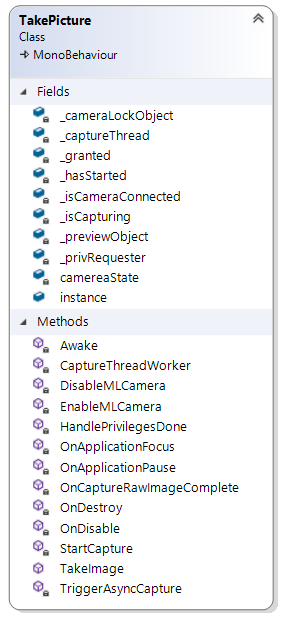
\includegraphics[width=0.4\textwidth]{images/dia_takepicture.PNG}
	\caption[]{Klassendiagramm TakePicture}
	\label{dia:takepicture}
\end{figure}

Das Script TakePicture implementiert das Aufnehmen von einem Foto.
Die Methode StartCapture wird aufgerufen, um den Prozess zu starten. 
MLCamera wird genutzt, um die Kamera der Magic Leap Brille anzusteuern.

%Image: Aufgenommenes Foto wird in AR UI angezeigt.

Wenn das Foto aufgenommen wurde, wird OnCaptureRawImageComplete aufgerufen. Die Daten des Bildes werden an die Klassen AzureObjectDetection und AzureCustomPrediction weitergegeben. Dort wird die Analyse der Bilder gestartet. 

\subsection{Object Detection}

\begin{figure}[H]
	\centering
	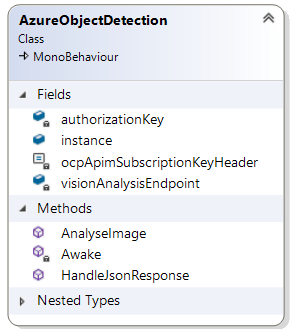
\includegraphics[width=0.4\textwidth]{images/dia_azureobjectdetection.PNG}
	\caption[]{Klassendiagramm AzureObjectDetection}
	\label{dia:azureobjectdetection}
\end{figure}

\begin{figure}[H]
	\centering
	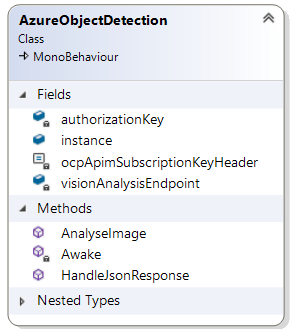
\includegraphics[width=0.4\textwidth]{images/dia_azureobjectdetection.PNG}
	\caption[]{Klassendiagramm AzureObjectDetection}
	\label{dia:azureobjectdetection}
\end{figure}

In der Methode AnalyseImage von AzureObjectDetection wird ein Post Web Request zusammengestellt, um die Azure REST API anzufragen. Der Request erhält einen Authentifizierung für die API und das zu analysierende Foto.

Der Webrequest wird verschickt und auf die Antwort gewartet. Wenn die Antwort eintrifft, wird anhand des ResponseCodes nachgeschaut, ob es bei dem Request einen Fehler gab. Beispielsweise kann die Internetverbindung gestört sein oder die Authentifizierung abgelehnt werden.
Wenn es keinen Fehler gab, wurde eine Json-Datei bei der Antwort mitgeschickt. Darin wird für jedes gefundene Objekt auf dem Foto eine Bezeichnung (Klasse) und eine Bounding Box angegeben. 

Die Json-Datei wird in HandleJsonResponse verarbeitet. Für den erwarteten Aufbau der Datei wurden drei Klassen geschrieben. Der Json String wird mit JsonUtility in ein DetectionResponse Object umgewandelt. Dabei werden alle gefundenen Foto-Objekte in einer Liste von DetectedObject abgelegt.\cite{fromjson}

Die gefundenen Objekte sollen im 3D Raum mit einer Markierung gekennzeichnet werden. 
Dafür wird für jedes DetectedObject die Methode Cast von der Klasse PixelToWorld aufgerufen. Der Methode wird der Mittelpunkt der BoundingBox als u,v Foto-Koordinate für das DetectedObject übergeben.

\subsection{Von dem Foto zum 3D Raum}

\begin{figure}[H]
	\centering
	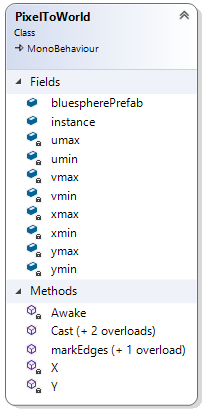
\includegraphics[width=0.3\textwidth]{images/dia_pixeltoworld.PNG}
	\caption[]{Klassendiagramm PixelToWorld}
	\label{dia:pixeltoworld}
\end{figure}

Das gefundene Foto-Objekt soll in der 3D Abbildung der realen Welt lokalisiert werden. Dafür nutzt die Methode Cast die u,v Foto-Koordinate des Objekts und die Kameraausrichtung.

Das Foto kann mit dem Display und somit mit der Clipping Plane der Hauptkamera approximiert werden.
Die u,v Foto-Koordinate wird zunächst in eine x,y,z Koordinate in dem Camera Space umgewandelt. Der z Anteil gibt die Entfernung von dem Ursprung der Kamera an in Blickrichtung an. Dabei befinden sich Punkte mit einer Entfernung von 0.4 Einheiten auf der Clipping Plane. In dem Camera Space mit z = -0.4 angegeben. 

Die x und y Dimensionen beschreiben die Achsen, die horizontal und vertikal zur Clipping Plane verlaufen. Mit dem festgelegten z = -0.4, kann jeder Punkt auf der Clipping Plane durch x und y angegeben werden. Dazu gehören auch Punkte die außerhalb des View Frustum liegen.

Es wurden Werte für x und y ausprobiert, mit denen die Ränder des Fotos auf der Clipping Plane angegeben werden können. Dabei wurde auf die unterschiedlichen Seitenverhältnisse des Fotos und des Displays geachtet. Darüber hinaus ist der Bildausschnitt des Displays kleiner. Daher liegen die Ränder des Fotos außerhalb des View Frustum. 

Sind diese x und y Werte bekannt, ergibt sich für die Achsen jeweils ein Intervall, die kombiniert alle Foto-Koordinaten auf die Clipping Plane abbilden können. Die Intervall lauten: [-0.295,0.2281] für x und [0.1546,-0.1507] für y. Mit den Intervallen wird die Position und Skalierung des Fotos in Relation zu dem Display - und der Hauptkamera - berücksichtigt. Siehe Kapitel \ref{section:devpixeltoworld} für die Entwickelung der Cast Methode und die Ermittlung der Intervallwerte.

Es werden zwei lineare Funktionen aufgestellt:
\begin{itemize}
	\item Die Funktion X bildet das Intervall für u [0,1920] auf das Intervall für x [-0.295,0.2281] ab.
	\item Die Funktion Y bildet das Intervall für v [0,1080] auf das Intervall für y [0.1546,-0.1507] ab.
\end{itemize}
Siehe Abbildung \ref{code:uvtoxy}.
\begin{figure}[H]
	\centering
	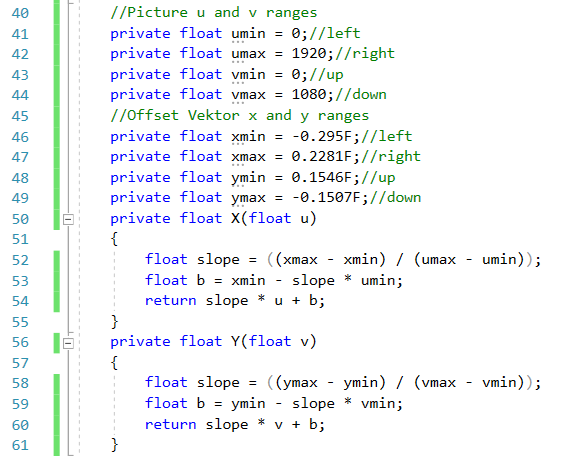
\includegraphics[width=0.6\textwidth]{images/code_uv_to_xy_scale.PNG}
	\caption[]{Funktionen X und Y}
	\label{code:uvtoxy}
\end{figure}

Mit den Funktionen wird eine Koordinate im Camera Space für u,v berechnet. Diese Koordinate wird dann, mithilfe der cameraToWorldMatrix, in die Koordinate p des globale Koordinatensystem umgewandelt. Damit wird die Position und Rotation der Kamera - und somit des Fotos - in der 3D Szene berücksichtigt. Siehe Abbildung \ref{code:castmethod}.

\begin{figure}[H]
	\centering
	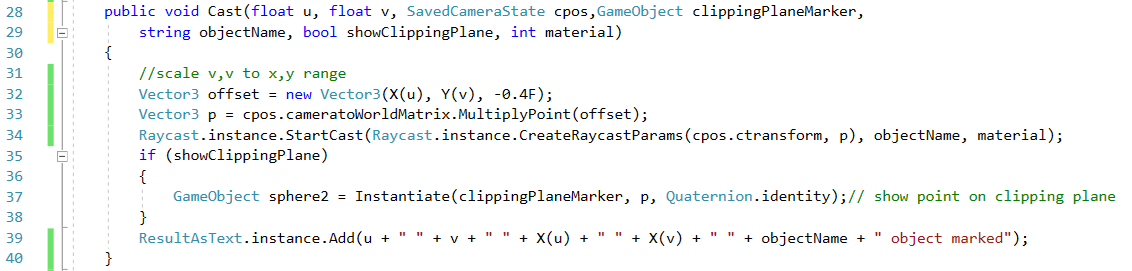
\includegraphics[width=1.2\textwidth]{images/code_cast_method.PNG}
	\caption[]{Cast Methode}
	\label{code:castmethod}
\end{figure}
\subsection{Raycast}

\begin{figure}[H]
	\centering
	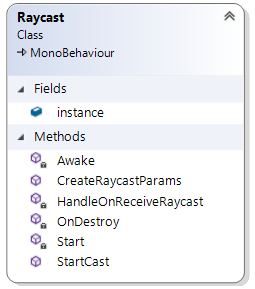
\includegraphics[width=0.3\textwidth]{images/dia_raycast.PNG}
	\caption[]{Klassendiagramm Raycast}
	\label{dia:raycast}
\end{figure}

Als Nächstes wird ein Raycast durch den Ursprung der Kamera und die Koordinate p gesendet. MLRaycast wird genutzt, um einen Schnittpunkt mit der Rekonstitution der Welt von Lumin OS zu bestimmen. Die Stelle, die der Raycast trifft beschreibt die Position des DetectedObject im 3D Raum.

Für den MLRaycast werden zwei Parameter benötigt:
\begin{itemize}
	\item Ein QueryParams Objekt, das Ursprung und Richtung für den Raycast beinhaltet.
	\begin{itemize}
		\item Ursprung: Kamera
		\item Richtung: Richtungsvektor von der Kamera zu der Koordinate p
	\end{itemize}
	\item Eine Methode die aufgerufen wird, wenn der Raycast fertig ist. 
		\begin{itemize}
		\item Callback Methode: HandleOnRecieveRaycast
	\end{itemize}
\end{itemize}

Siehe Abbildung \ref{code:raycastparams}.

\begin{figure}[H]
	\centering
	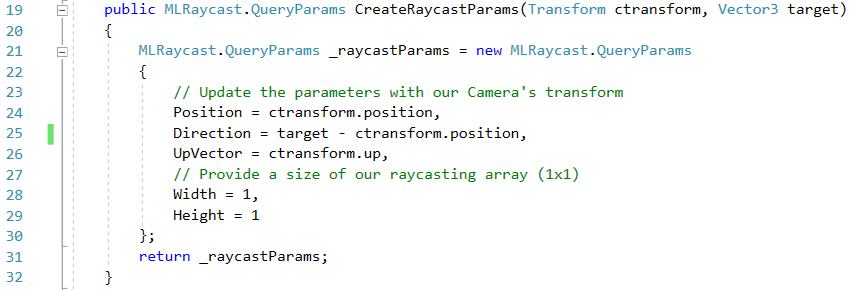
\includegraphics[width=0.9\textwidth]{images/code_raycastparams.PNG}
	\caption[]{Cast Methode}
	\label{code:raycastparams}
\end{figure}

Wenn der Raycast fertig ist, wird die Methode HandleOnRecieveRaycast aufgerufen. Der Parameter point beinhaltet dabei die getroffene Koordinate.
Diese wird an die Methode CreateMarker von der Klasse LabelCreater weitergegeben.

\subsection{LabelCreater}

CreateMarker erhält den Punkt point, der getroffen wurde und die Bezeichnung für das DetectedObject. An der Koordinate von point wird ein Prefab GameObject instanziiert, das als Markierung für das DetectedObject in der 3D Umgebung dient.

Das Prefab besteht aus einer Kugel und einem Schriftzug, der den Namen des DetectedObject anzeigen soll. Dem neu instanziierten GameObject wird die Bezeichnung des DetectedObject als Schriftzug zugewiesen. Siehe Abbildung \ref{image:labels}.

\begin{figure}[H]
	\centering
	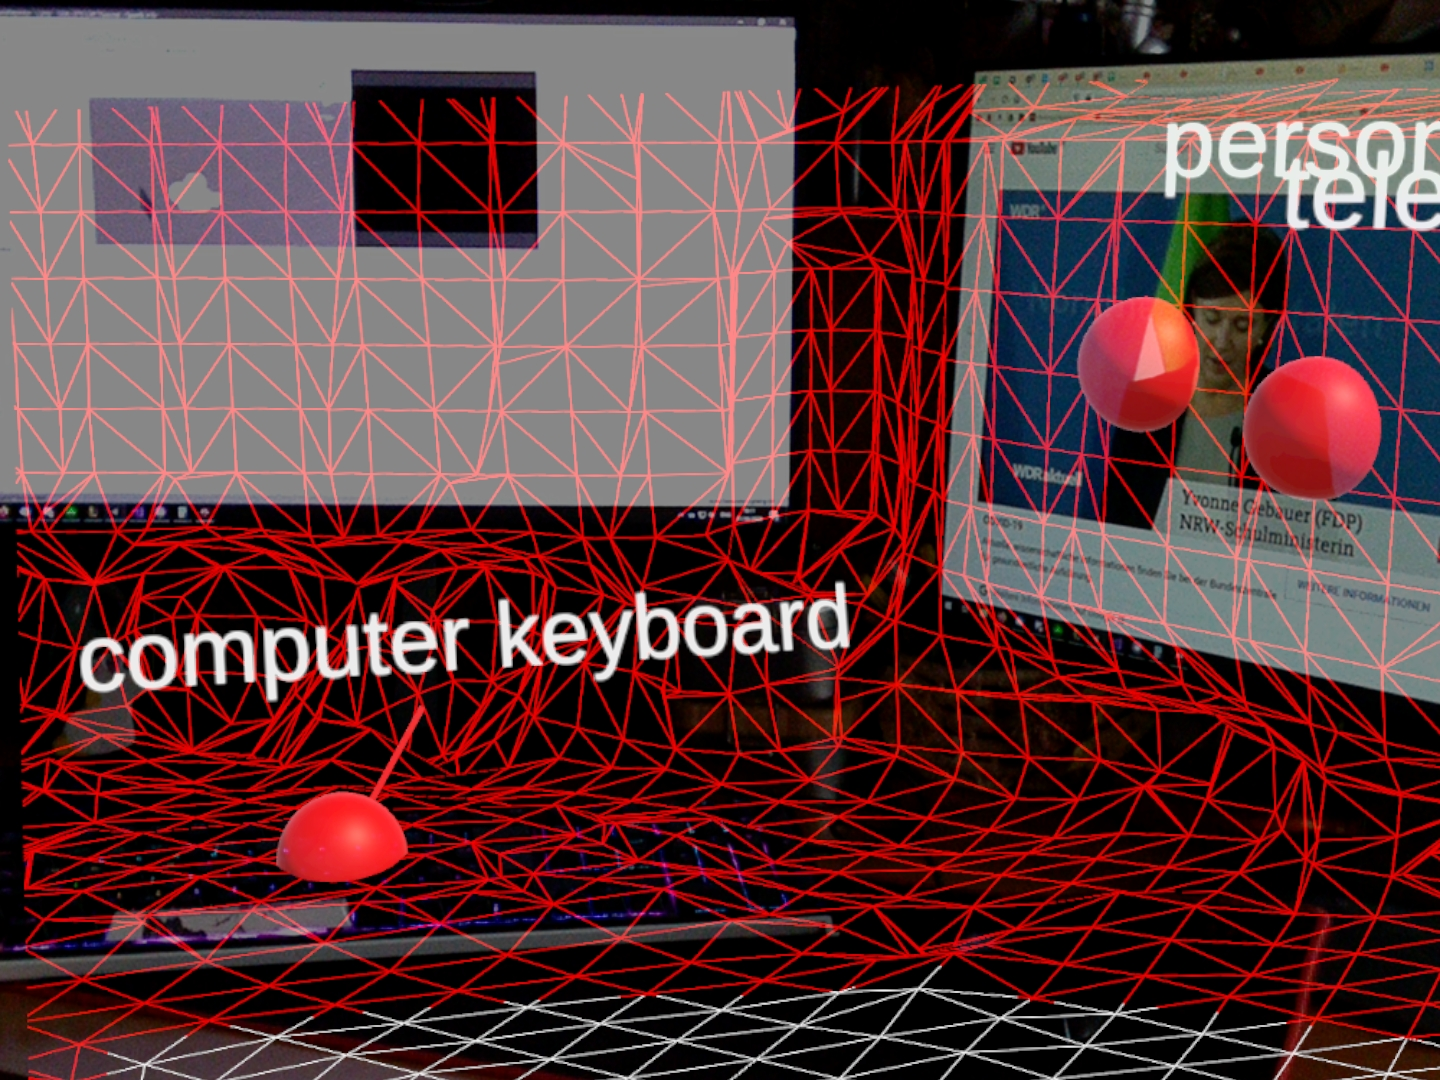
\includegraphics[width=0.7\textwidth]{images/ML_labels.jpg}
	\caption[]{Markierungen in der Welt}
	\label{image:labels}
\end{figure}

\subsection{Azure Custom Vision}

Neben der Bildanalyse mit Azure Object Detection wird auch Azure Custom Vision verwendet.
Die AI wurde über die Webseite trainiert.

Die Anfrage an den Service passiert in der Klasse AzureCustomPrediction. Ähnlich wie bei AzureObjectDetection wird ein Webrequest erstellt mit einem Authorization Key für den Service und einem Foto als Payload.

In der Antwort wird eine Json Datei zurückgeschickt, die die gefundenen Objekte angibt.
Da die Json Datei eine etwas anderes Format hat, wurde eine eigene HandleJsonResponse Methode dafür geschrieben.

Für jedes erkannte Objekt wird die Methode Cast von PixelToWorld aufgerufen, um das Objekt in der realen Welt zu lokalisieren und zu markieren.

\subsubsection{Das Trainieren}

Es wurde probiert das Custom Vision Modell auf drei unterschiedliche Objekte zu trainieren.
Dabei wurden vier Iterationen erstellt. 

Iteration 1:

Zunächst wurde probiert Tuben von Acrylfarbe zu erkennen. Die Genauigkeit davon war nicht sehr hoch. Es wurden in Fotos Acrylfarben an Stellen erkannt, an denen es keine gab. Siehe Abbildung \ref{image:customVisionPaint}. 

\begin{figure}[H]
	\centering
	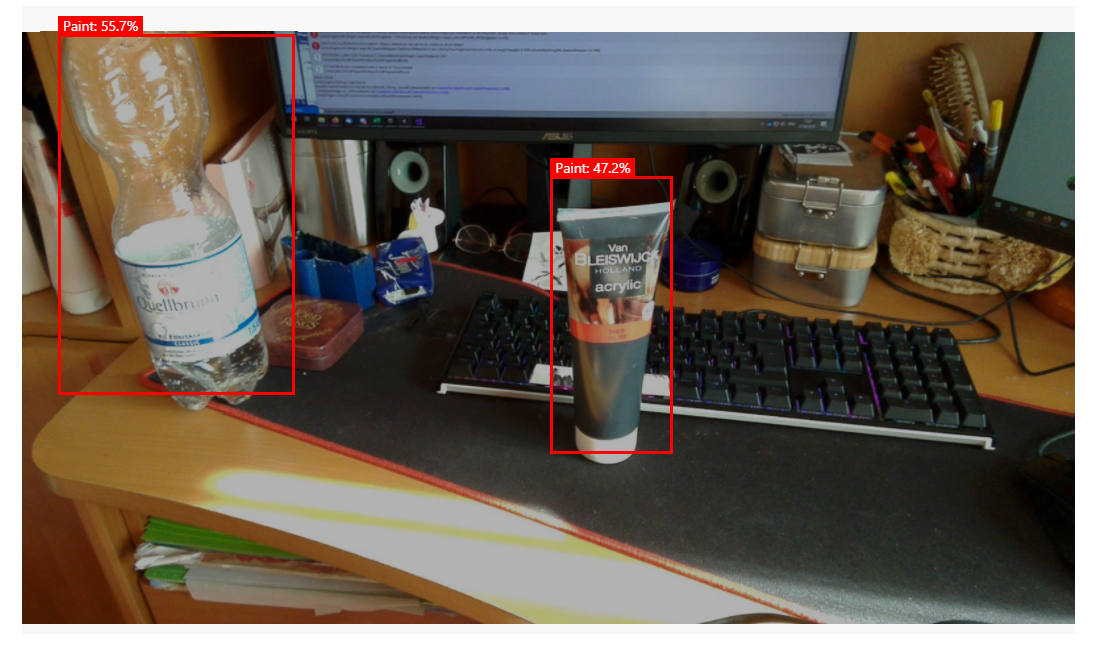
\includegraphics[width=1.0\textwidth]{images/customVisionPaint.PNG}
	\caption[]{Beispielfoto Iteration 1. Die Wasserflasche wurde als Farbe markiert mit 55.7 Prozent statistischer Konfidenz. Die Tatsächliche Farbtube wurde mit einer Konfidenz von 47.5 Prozent erkannt.}
	\label{image:customVisionPaint}
\end{figure}

Iteration 2:

In der zweiten Iteration wurde probiert das Modell darauf zu trainieren, eine blaue Dose von Nivea Hautcreme to erkennen. Die Form und Farbe der Dose ist sehr simpel, daher wurde davon ausgegangen, dass sie leichter zu erkennen ist. Die berechnete Prediction Wahrscheinlichkeit während des Trainings lag bei 80 Prozent.

Trotzdem wurden in vielen Fotos fälschlicherweise Nivea Dosen erkannt. 



Iteration 3:

In der dritten Iteration wurde versucht die vorherige Iteration zu verbessern. Es wurden ausgewählte Trainingsfotos entfernt, die die Dose von einem seitlichen Winkel zeigten. Die Erwartung war, dass die Detektion der Dose aus dem Blickwinkel von Oben konsistenter wird. Zusätzlich wurden mehr Fotos von der Dose auf unterschiedlich gefärbten und gemusterten Untergründen hinzugefügt. 

Die Genauigkeit der Prediction sank auf 75 Prozent.

Iteration 4:

In der vierten Iteration wurden zwei Fotos von der Nivea Dose entfernt, was die Genauigkeit auf 100 Prozent steigen ließ. In der Umsetzung mit der Magic Leap Anwendung wurden trotzdem häufig Objekte fälschlicherweise als Nivea Dose markiert.

Neben der Dose wurde diese Iteration darauf trainiert eine bestimmte Holzhaarbürste zu erkennen. Aufgrund von dem komplexeren, und markanten Aussehen der Bürste wurde davon ausgegangen, das die Bürste besser von anderen Objekte zu unterschieden ist. 
Die Bürste wurde nur mit den Borsten nach oben fotografiert.

Die Genauigkeit für die Bürste lag bei 100 Prozent. 
In der Umsetzung mit der Magic Leap Anwendung wird die Bürste häufig nicht erkannt, obwohl sie im Bild ist und mit den Borsten nach oben liegt. Es werden jedoch keine Objekte fälschlicherweise als Haarbürste erkannt.

\subsection{Entwicklung der Foto-Repräsentation}
\label{section:devpixeltoworld}

Um die u,v Foto-Koordinate eines gefundenen Objektes auf der Clipping Plane der Kamera zu lokalisieren, wurden ein paar Herangehensweisen ausprobiert.

Das Ziel ist das Setzten einer Markierung in dem 3D Raum, basierend auf der Foto-Koordinate. Das Foto beinhaltet keine Information über die Entfernung zu dem Objekt. Dafür muss ein Raycast durchgeführt werden. 

Mit einer Repräsentation des Fotos in dem 3D Raum ist es möglich diesen Raycast durchzuführen. 
Dazu muss das Foto nicht tatsächlich in dem 3D Raum vorhanden sein. Es muss jedoch mit dem Input einer Foto-Koordinate ein Output einer Koordinate in dem 3D Raum erzeugt werden, mit dem der Raycast durchgeführt werden kann.

Die Position des Fotos hängt mit der Kamera zusammen, daher kann das Foto durch den Camera Space simuliert werden. Als erstes wurde probiert ein Sphären-Objekt an eine gezielte Koordinate des Camera Space zu bewegen. 

% make pretty after this
Wenn die Kamera am Ursprung des globalen Koordinatensystem liegt und eine neutrale Rotation hat, stimmt der Camera Space mit dem globalen Koordinatensystem überein. Die Sphäre wurde in der Szene per Hand bewegt um markante Koordinaten des Camera Space abzulesen. Dabei wurden folgende Camera Space Koordinaten gefunden:
\begin{itemize}
	\item Near Clipping Plane bei z = -0.37
	\item linker Rand bei x = -0.153
	\item rechter Rand bei x = 0.153
	\item oberer Rand bei y = 0.1147
	\item unterer Rand bei y = -0.1147
\end{itemize}

Die x und y Koordinaten hängen von der u,v Koordinate des Fotos ab. Es wurden lineare Funktionen aufgestellt um u,v auf x,y abzubilden. Diese Abbildung dient als Repräsentation des Fotos im 3D Raum, unter Berücksichtigung der Position und Skalierung des Fotos im Verhältnis zu der Kamera.

Dann wurde getestet wie genau DetectedObjects in der AR Umgebung lokalisiert werden. Es wurden testweise Fotos aufgenommen, analysiert und die DetectedObjects markiert. Die entstandenen Markierungen lagen in Sichtfeld, jedoch nicht an den erwarteten Stellen. 

Um dem Problem auf den Grund zu gehen, wurde ein UI Objekt erstellt, das ein aufgenommenes Foto bei Runtime anzeigt.
Das Foto wurde dann mit dem Display verglichen. Dabei fiel auf, das sie ein unterschiedliches Seitenverhältnis haben und das Display einen kleinen Bildausschnitt zeigt.  

Es gibt zwei Möglichkeiten die Unterschiede zwischen Foto und Display auszugleichen. Entweder wird das Foto auf das Display zugeschnitten oder das gesamte Foto wird verwendet. Im zweiten Fall würden auch Objekte erkannt, die außerhalb des Sichtfeldes liegen.
Es wurde die Entscheidung getroffen das Foto zuzuschneiden. Damit gibt es ein besseres Feedback für den Nutzer, wenn ein Objekt gefunden wurde. 

Das Zuschneiden wurde realisiert, indem die Intervalle für u und v der Abbildungsfunktionen stärker eingegrenzt wurden. Alle Objekte die außerhalb der Intervalle liegen werden ignoriert. Um die Intervalle zu bestimmen wurde dem Fotoanzeige-UI-Element ein Gitter hinzugefügt. Mit dem Gitter kann die u,v Position von beliebigen Stellen des Fotos abgelesen werden. 
Durch Aufnehmen von Fotos und Vergleichen mit dem Sichtfeld des Displays wurde abgelesen, bei welcher u,v Position des Fotos die Ecken des Displays zu finden sind. Die Intervalle wurden dem entsprechend eingegrenzt. 

Mit den durchführten Veränderungen der Intervalle konnten DetectedObjects korrekt in der Umgebung lokalisiert werden. Jedoch wurden sehr häufig Objekte nicht markiert, obwohl sie im Sichtfeld des Nutzers lagen, weil deren Mittelpunkt außerhalb eines Intervalls lag.

Daher wurde entschieden die zweite Möglichkeit zu implementieren und das gesamte Foto zu verwenden und Objekte auch zu markieren, wenn sie komplett außerhalb des Sichtfeldes liegen. 
Dafür wurden die Intervalle für u und v wieder auf die ursprünglichen Werte - [0,1920] und [0,1080] - gesetzt. Die Intervalle für x und y mussten vergrößert werden.

Um die x und y Intervalle bestimmen zu können, wurde das Fotoanzeige-UI-Element Parallel zu der ClippingPlane gelegt. Das Element folgt den Bewegungen der Kamera und liegt möglichst nah an der Near Clipping Plane. Das Display der Magic Leap Brille zeigt selbst solide Objekte leicht durchsichtig an. Das wurde genutzt, um Fotos aufzunehmen, mit dem UI Element anzuzeigen und mit der realen Welt zu vergleichen. Durch Ausprobieren wurde das UI Element so skaliert und verschoben, dass das angezeigte Foto mit der realen Welt soweit wie möglich übereinstimmt.

Dann wurden die Ränder des UI Elementes genutzt um die Intervalle für x und y zu bestimmen.
\begin{itemize}
	\item für x: [-0.295, 0.2281]
	\item für y: [0.1546, -0.1507]
	\item Zusätzlich wurde z = -0.4 gesetzt. Das UI Element musste ein wenig weiter von der Clipping Plane entfernt sein um angezeigt zu werden.
\end{itemize}

Mit diesen Intervallen für u,v,x und y konnten DetectedObjects gut lokalisiert werden und es wurden keine Objekte mehr weggelassen, von denen der Nutzer erwarten würden, das sie markiert werden.


%bilder zeigen wie es dann aussieht
%make methods, classes and variables italic

\section{Zusammenfassung}
%sachen die verbessert werden könnten
%todo this part.

wie System auch für andere dinge verwendet werden kann. Beispielsweise Blindenführung und so
man kann zusätzlich zum Raycast auf die Spatial Map auch noch die Tiefentherapie nutzen. Spatial Mapping hat manchmal die Daten an der Stelle noch nicht, oder ist nicht aktualisiert. Besonders Probleme mit Wasserflaschen die nicht erkannt werden. Hinzuziehen von Tiefendaten kann das lokalisieren von Objekten im 3D Raum noch verbessern.

%Das Schätzen von der Anzahl an Haaren mithilfe von Bildverarbeitung und statistischer Auswertung zeigt sich als funktionsfähig und effizient. 
%In der Zukunft können die unterschiedlichen Schätzungs-Modelle miteinander verglichen werden, um die Kombination der akkuratesten Modelle zu finden. Die Genauigkeit sollte mit noch mehr Haar-Bildern getestet werden. 
%Der Bildverarbeitungsprozess braucht recht lange mit 20 bis 30 Sekunden pro Bild. Durch das weglassen von Daten die statistisch nicht ausgewertet werden, sowie das optimieren der Region-Untersuchungen kann der Prozess beschleunigt werden. 
	
\newpage
\printbibliography
\end{document}